\subsection{AR-HMM fails to identify interpretable behaviors in freely moving mice}
\label{sec:slds:3.2.2}

An AR-HMM is a popular model for capturing animal behavior because it assumes a linear relationship between the observations (joint positions) at one time point and those of the previous time point, thus capturing not just body pose but also temporal postural dynamics (Fig. \ref{fig:slds:2}a) \cite{wiltschko_mapping_2015, datta_computational_2019, datta_q_2019}. Mathematically this can be expressed as,
\begin{equation} \label{eq:slds_1}
y_t = w_{z_t}^T y_{t-1} + \epsilon \qquad \epsilon \sim \mathcal{N}(\mu,\sigma^2)
\end{equation}

\begin{figure}[t!]
  \begin{center}
    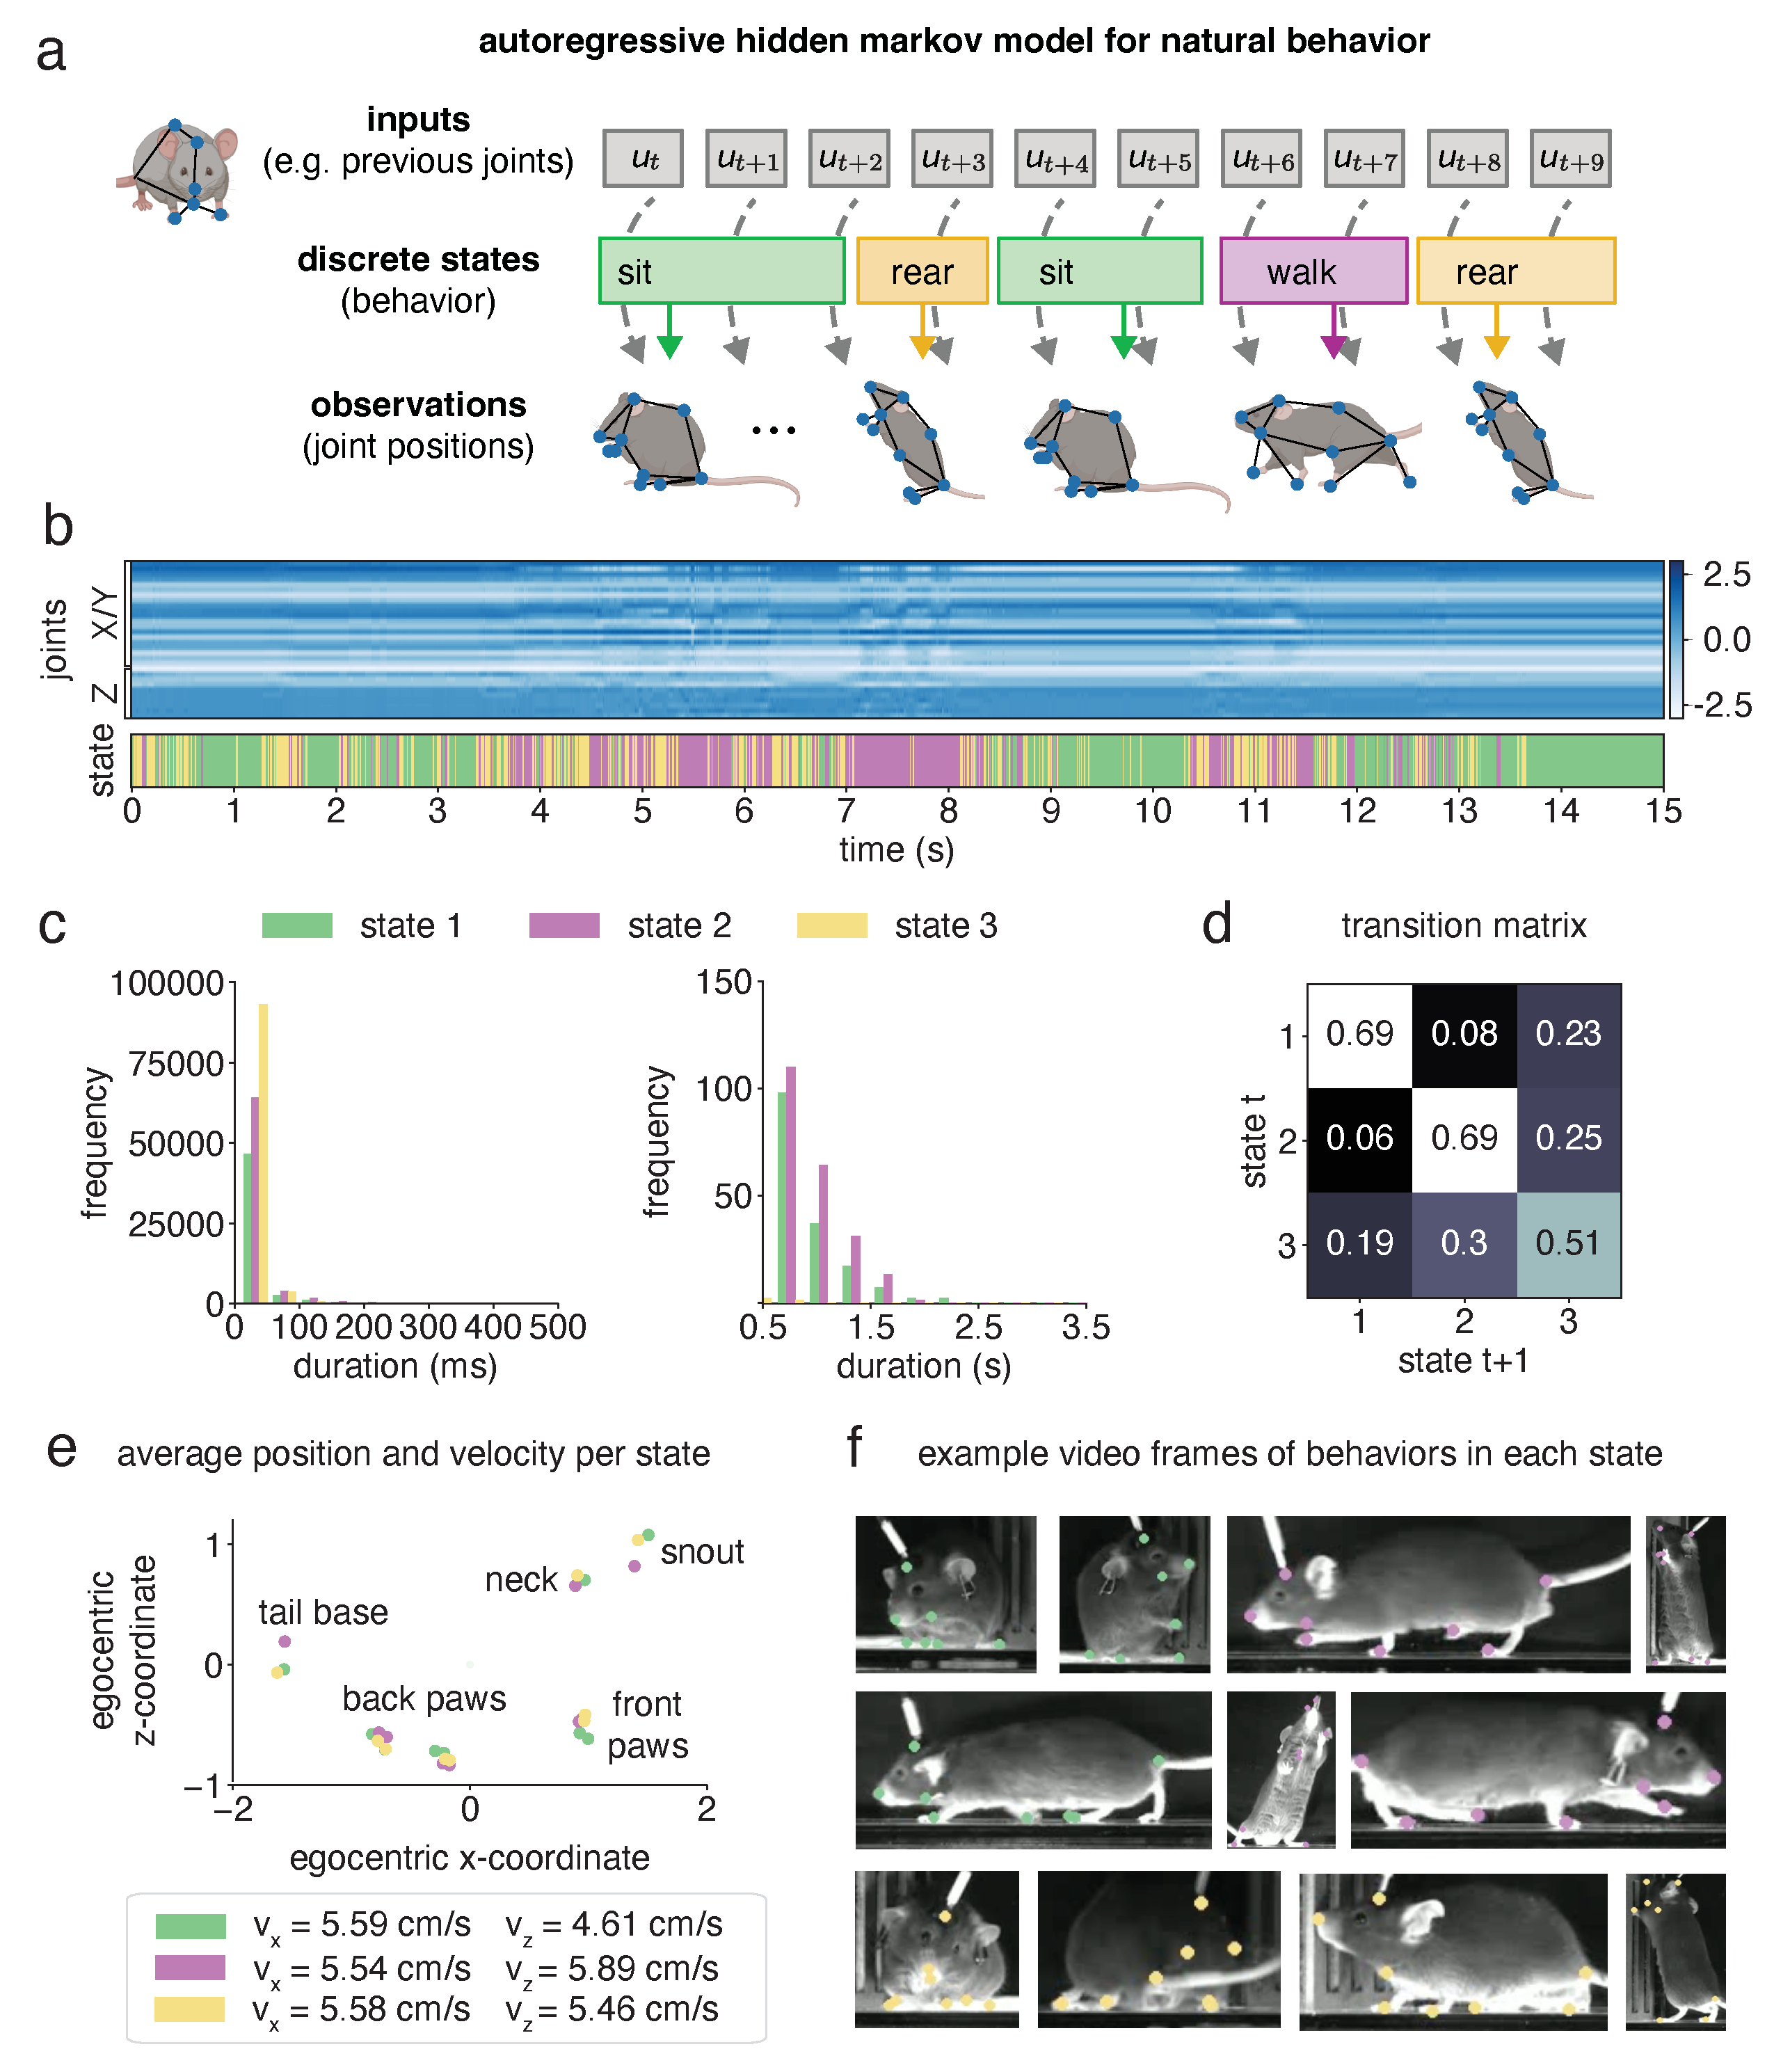
\includegraphics[width=0.90\linewidth]{ch3-slds/slds-figures/Fig2.pdf}
    \caption[Mouse body dynamics were tracked while they freely explored a linear track]{\textbf{Mouse body dynamics were tracked while they freely explored a linear track.} (a) Mice are placed into a linear track chamber with a slotted barrier on either end and a mirror underneath to provide two simultaneous views from one camera. Data are collected at 100Hz with high resolution. (b) Bottom and side body parts are tracked using SLEAP. Height information from 10 sideview body parts is z-scored. X and Y-coordinates of 10 bottomview body parts are centered, rotated, and z-scored. (c) Coordinates of side body parts (Z) is combined with bottomview coordinates (X/Y), and this combined dataset is the input to the model. }
    \label{fig:slds:2}
  \end{center}
  %\vspace{-1.5cm}
\end{figure}
where $y_t$ is the vector of observations at the current time point, $y_{t-1}$ is the vector of observations at the previous time point, $w$ is the model-inferred linear mapping between them, and $\epsilon$ is additive Gaussian noise with mean $\mu$ and covariance $\sigma^2$. For the purposes of consistency with the GLM-HMM described in Chapter \ref{ch:glmhmm}, in the schematic in Fig. \ref{fig:slds:2}a we have recast the previous joint positions as inputs such that $y_{t-1}=u_t$, but mathematically the details are as described in Equation \ref{eq:slds_1}. In addition to $w$, the AR-HMM learns a transition matrix that contains a fixed set of probabilities that govern the probability of changing from a state $z \in \{ 1, \ldots ,K\}$ on trial $t$ to any other state on the next trial. That is, 

\begin{equation}
\label{eq:slds_2}
    P_{ij} = p\left( {z_{t + 1} = j|z_t = i} \right)
\end{equation}

In the context of natural behavior, the goal of fitting the AR-HMM is typically to infer a set of $k$ states (with distinct weights $w$ associated with each one) that each represents a recognizable, stereotyped subset of an animal's broader behavioral repertoire, such as sitting, walking, or rearing (Fig. \ref{fig:slds:2}a).

While this approach works well when the observations are smoothly-varying data points acquired from depth-imaging cameras \cite{wiltschko_mapping_2015, markowitz_striatum_2018, wiltschko_revealing_2020}, the results are far less promising when the observations are keypoints. In fitting a 3-state AR-HMM with the objective of capturing the three most fundamental behaviors that a mouse can exhibit in the linear track chamber, we found that the inferred states tend to ``flicker" back and forth rapidly in a manner that does not correspond to synchronized changes in the joint positions (Fig. \ref{fig:slds:2}b, note in particular the sudden change in the value of the majority of the joint positions between 10 and 12 seconds that is not captured by the inferred state sequence) and the state durations tend to be much shorter than the average $\sim$350ms for many behaviors that has been reported elsewhere (Fig. \ref{fig:slds:2}c, mean=46.9ms, median=20ms) \cite{wiltschko_mapping_2015}. The inferred transition matrix reflects this feature of the state sequences as well, with a weakly diagonal structure that indicates nearly as high a likelihood of transitioning into another state as staying in the same state from one trial to the next (Fig. \ref{fig:slds:2}d). 

Not only are the AR-HMM inferred states unusually short, they also do not correspond to interpretable, distinct behaviors. Neither the average keypoint positions nor the average velocity (computed by taking the difference in successive keypoint positions for the uncentered, unrotated data) from frames assigned to each state are distinguishable from one another (Fig. \ref{fig:slds:2}e). In addition, across all videos there are instances where the model assigns each state to all manner of rearing, sitting, and walking actions, indicating little consistent relationship between the inferred states and specific behaviors. 

One likely reason that the AR-HMM failed to identify states of sufficient duration is that there is noise in the keypoint data. Manual inspection of videos revealed a high-frequency ``jitter" in the joint position assignments that was not associated with observable changes in the animals' poses. Rather, the jitter appeared to be attributable to the keypoint tracking software itself and was a function of uncertainty in the correct positional assignments and/or occasional body part occlusions (e.g. when the mouse turned away from the camera or stuck his snout through one of the slotted barriers). It is possible that the AR-HMM interpreted these sudden jumps in the joint positions as true behavioral changes, leading to short, uninterpretable states. Attempts to resolve this problem by labeling more frames in order to increase the certainty in the keypoint assignments from SLEAP generated minimal improvements, as did efforts to subsequently smooth the keypoint data using filters, interpolation, and other techniques. 